\documentclass[11pt,a4paper]{article}

% ---- packages ----
\usepackage[T1]{fontenc}
\usepackage[utf8]{inputenc}
\usepackage{amsmath,amssymb,amsthm}
\usepackage{mathtools}
\usepackage[dvipsnames]{xcolor}
\usepackage[colorlinks=true,linkcolor=NavyBlue,citecolor=ForestGreen,urlcolor=NavyBlue]{hyperref}
\usepackage{booktabs}
\usepackage{array}
\usepackage{geometry}
\geometry{margin=2.5cm}
\usepackage{enumitem}
\usepackage{graphicx}
\usepackage{doi}

% ---- theorem environments ----
\theoremstyle{plain}
\newtheorem{theorem}{Theorem}[section]
\newtheorem{proposition}[theorem]{Proposition}
\newtheorem{lemma}[theorem]{Lemma}
\newtheorem{corollary}[theorem]{Corollary}
\newtheorem{conjecture}[theorem]{Conjecture}

\theoremstyle{definition}
\newtheorem{definition}[theorem]{Definition}
\newtheorem{example}[theorem]{Example}

\theoremstyle{remark}
\newtheorem{remark}[theorem]{Remark}

% ---- hyperref configured above ----

% ---- macros ----
\newcommand{\F}{\mathbb{F}}
\newcommand{\R}{\mathbb{R}}
\newcommand{\C}{\mathbb{C}}
\newcommand{\Z}{\mathbb{Z}}
\newcommand{\N}{\mathbb{N}}
\newcommand{\Cl}{\mathrm{Cl}}
\newcommand{\rank}{\operatorname{rank}}
\newcommand{\PSL}{\mathrm{PSL}}
\newcommand{\adm}{\mathrm{adm}}
\newcommand{\Gadm}{\widehat{G}^{\adm}}
\newcommand{\Madm}{M_{\adm}}
\newcommand{\PiA}{\Pi_A}
\newcommand{\PiB}{\Pi_B}
\newcommand{\dA}{\partial^A}
\newcommand{\dB}{\partial^B}
\newcommand{\kap}{\kappa_\rho}
\DeclareMathOperator{\rowspan}{rowspan}
\DeclareMathOperator{\End}{End}
\newcommand{\rtildeB}{\tilde{r}_n^{B,\mathrm{mat}}}
\newcommand{\betaeff}{\beta_{\mathrm{eff}}}
\newcommand{\betastar}{\beta^*}
\newcommand{\betaprod}{\beta_{\mathrm{prod}}}
\newcommand{\piA}{\pi_A}
\newcommand{\piB}{\pi_B}
\newcommand{\PiBn}[1]{\Pi_B^{<#1}}

\begin{document}

  \title{%
    Admissible Frontier Saturation and the Cascade Exponent:\\
    A Representation-Theoretic Obstruction and its Matrix-Level Refinement%
  }

  \author{%
    J\'er\^ome Beau\\[4pt]
    \small Independent Researcher; \texttt{jerome.beau@cosmochrony.org}%
  }

  \date{March 2026}

  \maketitle

  \begin{abstract}
    The Cosmochrony relaxation cascade generates an inter-generational mass hierarchy through
    the contraction of the Kesten--McKay spectral support as the effective valence $p(n)$ grows.
    The cascade exponent $\beta$ governing $p(n) \sim n^\beta$ was identified in companion papers
    as the sole remaining structural parameter of the admissibility sub-programme: O3 constrains
    $\betastar \in (0.09, 0.13)$ from lepton masses, while O4 derives the quadratic upper bound
    $p(n) \lesssim Cn^2$ from bounded-flux and Cheeger arguments, leaving a factor of
    $10$--$20$ unexplained.

    The present paper introduces the notion of \emph{admissible frontier}: the subset of the raw
    BFS boundary whose elements introduce genuinely new directions in the admissible spectral
    subspace.
    We prove that the vertex-based admissible span $\mathcal{R}_A = \mathrm{span}\{\pi_A(g) : g \in
    G\}$ has dimension $r_A \le \rank(M_{\adm}) \le |\Cl(G)| = O(q)$, far below $|G| = O(q^3)$, by a
    direct consequence of the representation theory of $G = \PSL(2, \F_q)$.
    This gives the existence of a finite spanning witness $T \subset G$ with $|T| = r_A$ and
    $\Pi_A(T) = \mathcal{R}_A$ --- a statement about the abstract dimension of the admissible span,
    not about how quickly a graph exploration reaches such a witness.
    An explicit BFS run on $X^{5,13}$ needs far more than $r_A$ vertices to span $\mathcal{R}_A$,
    illustrating that gap concretely.

    We then examine transition-based refinements, using a shell-layered definition of transitional
    novelty in which the transitions entering graph-distance shell $n$ are tested only against the
    span of strictly earlier shells, avoiding both the self-reference of a naive definition and any
    dependence on BFS traversal order.
    Character-based transition fingerprints collapse to a fixed, low-dimensional span well below the
    admissible ambient dimension on LPS graphs, where all generators lie in a single conjugacy
    class.
    Fixed-dimensional matrix proxies saturate their own ambient dimension after a handful of shells,
    disqualifying them as structural mechanisms.
    A Steinberg-based fingerprint using the permutation action on $\mathbb{P}^1(\F_q)$ saturates its
    full $O(q)$-dimensional ambient space within the first two to three graph-distance shells for
    every tested $q \in \{13, 17, 29\}$ --- before the local tree-like regime around the origin gives
    way to genuine cycles --- leaving no usable pre-saturation window from which to extract an
    effective exponent.

    None of the constructions examined here yields a viable mechanism for the smallness of
    $\betastar$.
    A conjectural matrix-level redundancy law proposed in an earlier version of this paper is
    withdrawn as a candidate mechanism: it shares its functional form with the expander-derived
    conversion law shown by the companion Span-Growth Note not to transfer natively to a different
    admissibility substrate, and the present shell-layered numerics supply no pre-saturation regime
    in which such a law could even be measured.
    The paper's positive content is confined to what is proved: the dimension bound on the
    vertex-based admissible span, and a set of $q$-finite numerical observations about the tested
    transition-based fingerprints, none of which currently constitutes a structural derivation of
    $\betastar$.
  \end{abstract}

  \textbf{Keywords:} admissible frontier; cascade exponent; $\PSL(2,\F_q)$;
  LPS Ramanujan graphs; Kesten--McKay measure; representation theory; Steinberg representation;
  mass hierarchy; spectral admissibility.

  \clearpage
  \tableofcontents
  \bigskip\hrule\bigskip

  \clearpage

  \section{Introduction}
    \label{sec:introduction}

    \subsection{Background and motivation}

      The Cosmochrony framework~\cite{Cosmochrony} posits that physical observables arise through
      a non-injective projection $\Pi\colon \Omega_\chi \to \mathcal{O}$, where $\Omega_\chi$ is a
      pre-geometric relational substrate.
      The non-injectivity is not a defect but a structural feature motivating bounded projective
      capacity, emergent gauge structure, and finite resolution~\cite{Beau2026c}.

      Effective particle masses emerge from the relaxation dynamics on $\Omega_\chi$, organised into
      a discrete cascade indexed by rank $n$.
      At each rank, the connectivity of the substrate is encoded in a Ramanujan--LPS Cayley graph
      $G(n) = X^{p(n),q}$ of degree $d(n) = p(n)+1$, where $p(n)$ is the effective valence
      parameter~\cite{Beau2026a6}.
      As $p(n)$ grows, the Kesten--McKay spectral support contracts toward $\lambda = 1$, causing
      fixed ADE eigenvalue levels to exit the support at distinct cascade ranks and generating the
      observed mass ordering~\cite{Beau2026a7}.

      The inter-generational mass ratios are governed by
      \begin{equation}
        \label{eq:mass-ratio}
        \frac{M_i}{M_j} \approx
        \left(\frac{|\lambda_i - 1|}{|\lambda_j - 1|}\right)^{2/\beta},
      \end{equation}
      where $\lambda_i$ are fixed ADE eigenvalues and $\beta$ is the exponent in $p(n) \sim n^\beta$~\cite{Beau2026a7}.
      Matching~\eqref{eq:mass-ratio} to the charged lepton hierarchy yields
      $\betastar \in (0.09, 0.13)$, but leaves $\beta$ as a phenomenological input.

    \subsection{What O4 establishes and what remains open}

      The companion paper O4~\cite{Beau2026a8} shows that the bounded-flux constraint
      $|\partial_t \chi_v| \le c_{\mathrm{BI}}$, the capacity axiom [A-cap] of~\cite{Beau2026c},
      limits the advance of the exploration front:
      \begin{equation}
        \label{eq:O4-front}
        \Delta p(n) \lesssim c_{\mathrm{BI}} \sqrt{p(n)},
      \end{equation}
      which integrates to
      \begin{equation}
        \label{eq:O4-quad}
        p(n) \lesssim \tfrac{1}{4} c_{\mathrm{BI}}^2 \, n^2.
      \end{equation}
      Under the convention $p(n) \sim n^\beta$, this implies $\beta \le 2$ algebraically.
      The tighter claim $\beta \le 1$ of~\cite{Beau2026a8} identifies the saturated case as the
      maximal growth rate and restricts attention to $\beta \in (0,1]$.
      In either convention, the factor of $10$--$20$ between this bound and the phenomenological
      window $\betastar \approx 0.1$ is left unexplained.

      The present paper is O5 in the series.
      Its objective is to identify which mechanisms can and cannot bridge this gap.

    \subsection{Main results}

      The central contributions are the following.

      \textbf{Theorem (Proposition~\ref{prop:vertex-admissible-saturation}).}
      The vertex-based admissible span $\mathcal{R}_A = \Pi_A(G)$ has dimension
      $r_A \le \rank(\Madm) \le |\Cl(G)| = O(q)$, far below $|G| = O(q^3)$.
      Consequently there is a finite spanning witness $T \subset G$ with $|T| = r_A$ and
      $\Pi_A(T) = \mathcal{R}_A$, so $\dA S = \varnothing$ for every $S \supseteq T$.
      This is an existence statement about the abstract admissible span; it gives no bound on how
      many vertices a graph exploration must visit before encountering such a witness, which is
      audited numerically and found to be substantially larger than $r_A$ in practice
      (Remark~\ref{rem:numerical-A}).

      \textbf{Negative structural results (Section~\ref{subsec:transition-frontier}).}
      Under the shell-layered transitional frontier of
      Definition~\ref{def:transition-fingerprint}, character-based transition fingerprints collapse
      to a fixed, low-dimensional span well short of the admissible ambient dimension, and
      fixed-dimensional matrix proxies saturate their own ambient dimension almost immediately.
      The Steinberg-based fingerprint on $\mathbb{P}^1(\F_q)$ saturates its full $O(q)$-dimensional
      ambient space within the first two to three graph-distance shells for every tested
      $q \in \{13,17,29\}$, leaving no pre-saturation window from which any effective exponent could
      be extracted (Section~\ref{subsec:contributions-summary}).

      \textbf{Withdrawn candidate mechanism (Section~\ref{subsec:structural-implications}).}
      An earlier version of this paper proposed a conjectural matrix-level redundancy law linking a
      transitional-frontier decay rate to $\betaeff$.
      That conjecture is withdrawn as a candidate mechanism: no construction examined here supplies
      the required pre-saturation regime, and the conjectured law shares its functional form with an
      expander-derived conversion law shown elsewhere in the corpus not to transfer natively to a
      different admissibility substrate (Remark~\ref{rem:conjecture-withdrawn}).

    \subsection{Organisation}

      Section~\ref{sec:admissible-frontier} introduces the admissible frontier and proves
      Proposition~\ref{prop:vertex-admissible-saturation}.
      The transition-based refinements are developed and tested numerically in
      Sections~\ref{subsec:transition-frontier}--\ref{subsec:contributions-summary}.
      Section~\ref{subsec:structural-implications} derives the structural lesson, and
      Section~\ref{subsec:outlook-O6} states the conclusion and opens the next programme.

  \section{Admissible Frontier Saturation}
    \label{sec:admissible-frontier}


    The central difficulty identified in~\cite{Beau2026a8} is the following.
    The LPS Cayley graph $X^{p,q}$ is Ramanujan: its combinatorial expansion is optimal, and the
    raw boundary $|\partial S_n|$ grows robustly along any BFS cascade.
    Yet the argument of~\cite{Beau2026a8} establishes only the quadratic upper bound
    \begin{equation}
      \label{eq:O4-bound}
      p(n) \lesssim \tfrac{1}{4} c_{\mathrm{BI}}^2 \, n^2,
    \end{equation}
    derived by integrating $\Delta p(n) \lesssim c_{\mathrm{BI}}\sqrt{p(n)}$ under the closure hypothesis
    $p(n) \propto N(n)$.
    Under the convention $p(n) \sim n^\beta$ of the O-series~\cite{Beau2026a7,Beau2026a8},
    this implies $\beta \le 2$ algebraically.
    The tighter formulation $\beta \le 1$ of~\cite{Beau2026a8} identifies the saturated case as
    the maximal admissible growth rate; we adopt this convention here.
    In either interpretation, the bound leaves the phenomenological window
    $\betastar \in (0.09, 0.13)$ of~\cite{Beau2026a7} unexplained by a factor of $10$--$20$.
    The gap cannot be closed by refining the Cheeger bound alone, since the Ramanujan property
    of $X^{p,q}$ implies that Cheeger constants are already near-optimal for the graph
    combinatorics.

    \begin{remark}[Decoupling from the O4 normalisation]
      \label{rem:O4-decoupling}
      The quadratic bound $p(n) \lesssim C n^2$ is the only statement used from~\cite{Beau2026a8}
      in the present work.
      Any further normalisation of $\beta$ is purely conventional and does not affect the arguments
      below.
    \end{remark}

    The resolution proposed here is that the relevant quantity is not the raw boundary $\partial S_n$
    but the \emph{admissibly productive} boundary: the subset of $\partial S_n$ whose elements
    introduce genuinely new directions in the admissible spectral subspace.
    We show that, at the vertex level, this notion of novelty is confined to an abstract span of
    dimension $r_A = O(|\Cl(G)|) \ll |G|$, independently of the graph's combinatorial expansion,
    and that a finite witness set of exactly that size exists.
    How large a set an actual graph exploration must visit before finding such a witness is a
    separate question, audited numerically below and found to be substantially larger than $r_A$.

    \subsection{Admissible sectors and the character matrix}
      \label{subsec:admissible-sectors}

      Let $G = \PSL(2, \F_q)$ with LPS generating set $\mathcal{S}_p \subset G$ of cardinality
      $d = p + 1$.
      We recall from~\cite{Beau2026a1} that the bounded-flux constraint
      $|\partial_t \chi_v| \le c_{\mathrm{BI}}$ induces a spectral admissibility envelope
      \begin{equation}
        \label{eq:admissibility-envelope}
        A_\rho^{\max} = \frac{c_{\mathrm{BI}}}{\sqrt{\lambda_\rho}},
      \end{equation}
      where $\lambda_\rho = d - \mu_\rho$ is the Laplacian eigenvalue of the irreducible sector
      $\rho \in \widehat{G}$.
      The sector $\rho$ is \emph{admissible} if $0 < \lambda_\rho \le \lambda^*$, where
      $\lambda^* = (\sqrt{d-1}+1)^2$ is the Ramanujan spectral bound~\cite{Beau2026a1}.
      We write $\Gadm \subset \widehat{G}$ for the set of admissible sectors.

      \begin{definition}[Admissible character matrix]
        \label{def:admissible-character-matrix}
        The \emph{admissible character matrix} is
        \[
          \Madm \in \R^{|\Cl(G)| \times |\Gadm|},
          \qquad
          (\Madm)_{[g], \rho} := \chi_\rho(g),
        \]
        where $[g]$ denotes the conjugacy class of $g$ and $\chi_\rho$ is the character of $\rho$.
        Rows are indexed by conjugacy classes; columns by admissible sectors.
      \end{definition}

      \begin{remark}[Dimensions]
        \label{rem:dimensions}
        For $G = \PSL(2,\F_q)$ with $q$ an odd prime:
        $|G| = q(q^2-1)/2 = O(q^3)$;
        $|\Cl(G)| = O(q)$;
        $|\Gadm| \le |\widehat{G}| = O(q)$.
        Hence $\Madm$ is $O(q) \times O(q)$ and $\rank(\Madm) \le |\Cl(G)| = O(q)$,
        while the group itself has order $O(q^3)$.
      \end{remark}

    \subsection{The vertex-based admissible fingerprint}
      \label{subsec:vertex-fingerprint}

      \begin{definition}[Vertex-based admissible fingerprint]
        \label{def:vertex-fingerprint}
        For $g \in G$, the \emph{vertex-based admissible fingerprint} is
        \[
          \piA(g) := \bigl(\kap \, \chi_\rho(g)\bigr)_{\rho \in \Gadm}
          \in \R^{|\Gadm|},
        \]
        where $\kap = \mu_\rho / d$ is the normalised adjacency eigenvalue
        (\emph{spectral coupling},~\cite{Beau2026a2}).
        For $S \subseteq G$ define
        \[
          \PiA(S) := \mathrm{span}_{\R}\{\piA(g) : g \in S\}
          \subseteq \R^{|\Gadm|},
        \]
        and the \emph{vertex-based admissible frontier}
        $\dA S := \{v \in \partial S : \piA(v) \notin \PiA(S)\}$.
      \end{definition}

    \subsection{Rapid saturation of the vertex-based admissible span}
      \label{subsec:saturation}

      \begin{proposition}[Dimension bound and finite spanning witness]
        \label{prop:vertex-admissible-saturation}
        Let $G = \PSL(2, \F_q)$, $\Gadm$ the admissible sectors, and $\piA$, $\PiA(S)$, $\dA S$
        as in Definition~\ref{def:vertex-fingerprint}.
        Define the vertex-based admissible span and its dimension
        \begin{equation}
          \label{eq:RA-def}
          \mathcal{R}_A := \PiA(G) = \mathrm{span}_\R\{\piA(g) : g \in G\},
          \qquad
          r_A := \dim \mathcal{R}_A.
        \end{equation}
        Then
        \begin{equation}
          \label{eq:rank-bound}
          r_A \le \rank(\Madm) \le |\Cl(G)|.
        \end{equation}
        Consequently there exists a finite spanning witness $T \subset G$ with $|T| = r_A$ such that
        $\PiA(T) = \mathcal{R}_A$, and
        \begin{equation}
          \label{eq:frontier-empty}
          \dA S = \varnothing
          \qquad \text{for every } S \supseteq T.
        \end{equation}
      \end{proposition}

      \begin{proof}
        For every $g \in G$, the character $\chi_\rho(g)$ is a class function depending only on
        $[g] \in \Cl(G)$.
        Hence $\piA(g)$ is constant on each conjugacy class, and $\mathcal{R}_A = \PiA(G)$ is
        contained in the row space of $\Madm$, giving $r_A \le \rank(\Madm) \le |\Cl(G)|$.
        Since $\mathcal{R}_A$ is a finite-dimensional space spanned by $\{\piA(g) : g \in G\}$, this
        spanning family contains a basis of size $r_A$; let $T \subset G$ be a corresponding set of
        group elements, so $|T| = r_A$ and $\PiA(T) = \mathcal{R}_A$.
        For every $v \in G$, $\piA(v) \in \mathcal{R}_A = \PiA(T)$ by definition of $\mathcal{R}_A$;
        hence $\piA(v) \in \PiA(S)$ for every $S \supseteq T$, so $\dA S = \varnothing$.
      \end{proof}

      \begin{remark}[The witness is existential, not algorithmic]
        \label{rem:witness-existential}
        The proof extracts $T$ from finite-dimensional linear algebra: any spanning family of a
        space of dimension $r_A$ contains a basis of size $r_A$.
        It gives no information about \emph{which} $r_A$ elements of $G$ form such a basis, nor
        about how many vertices a graph traversal --- BFS or any other order --- must visit before
        its accumulated set happens to span $\mathcal{R}_A$.
        The two questions are logically independent, and are kept separate throughout: the
        proposition settles only the first.
        Remark~\ref{rem:numerical-A} audits the second numerically and finds it is not tight.
      \end{remark}

      \begin{corollary}[Finite bound on the rank-to-size ratio]
        \label{cor:productivity-bound}
        For any nested family $S_1 \subseteq S_2 \subseteq \cdots \subseteq G$ (in particular the
        cumulative sets $(S_n)$ of a BFS cascade on $X^{p,q}$), $\PiA(S_n) \subseteq \mathcal{R}_A$
        for every $n$, so
        \begin{equation}
          \label{eq:rn-bound}
          r_n := \frac{\dim \PiA(S_n)}{|S_n|} \le \frac{r_A}{|S_n|}.
        \end{equation}
        Because $G$ is finite, this is a bound on the finite range $1 \le |S_n| \le |G|$, not an
        asymptotic statement: as $S_n$ exhausts $G$, $r_n$ decreases toward the strictly positive
        floor $r_A/|G|$, never to $0$, at fixed $q$.
        A genuine vanishing limit $r_n \to 0$ would require a separate family limit $q \to \infty$
        together with a controlled growth rate for $|S_n|$ as a function of $q$; this is not pursued
        in the present paper.
        Once $S_n \supseteq T$ for the witness $T$ of Proposition~\ref{prop:vertex-admissible-saturation},
        $\dA S_n = \varnothing$; by finiteness of $G$ this occurs at some finite $n$, but the
        proposition provides no bound on $|S_n|$ at that point beyond the trivial $|S_n| \le |G|$.
      \end{corollary}

      \begin{remark}[Numerical observation --- traversal-dependent, not a bound]
        \label{rem:numerical-A}
        For $G = \PSL(2, \F_{13})$ with $p = 5$, $d = 6$: $|G| = 4368$, $|\Gadm| = 12$,
        $\rank(\Madm) = r_A = 5$.
        On the graph-distance shells of $X^{5,13}$ from a fixed origin vertex (shell sizes
        $1, 6, 26, 116, 410, \ldots$), the cumulative vertex-based span $\PiA(S_n)$ reaches dimension
        $r_A = 5$ only once $|S_n| = 149$ --- nearly thirty times the abstract minimum $r_A = 5$
        guaranteed by Proposition~\ref{prop:vertex-admissible-saturation}.
        This is an empirical property of this specific exploration order, not a general bound:
        the proposition guarantees only the existence of \emph{some} witness of size $r_A$, with no
        guarantee that a natural exploration order finds one quickly, exactly as flagged in
        Remark~\ref{rem:witness-existential}.
        See Figure~\ref{fig:O5-A-vs-B}.
      \end{remark}

      \begin{figure}[ht]
        \centering
        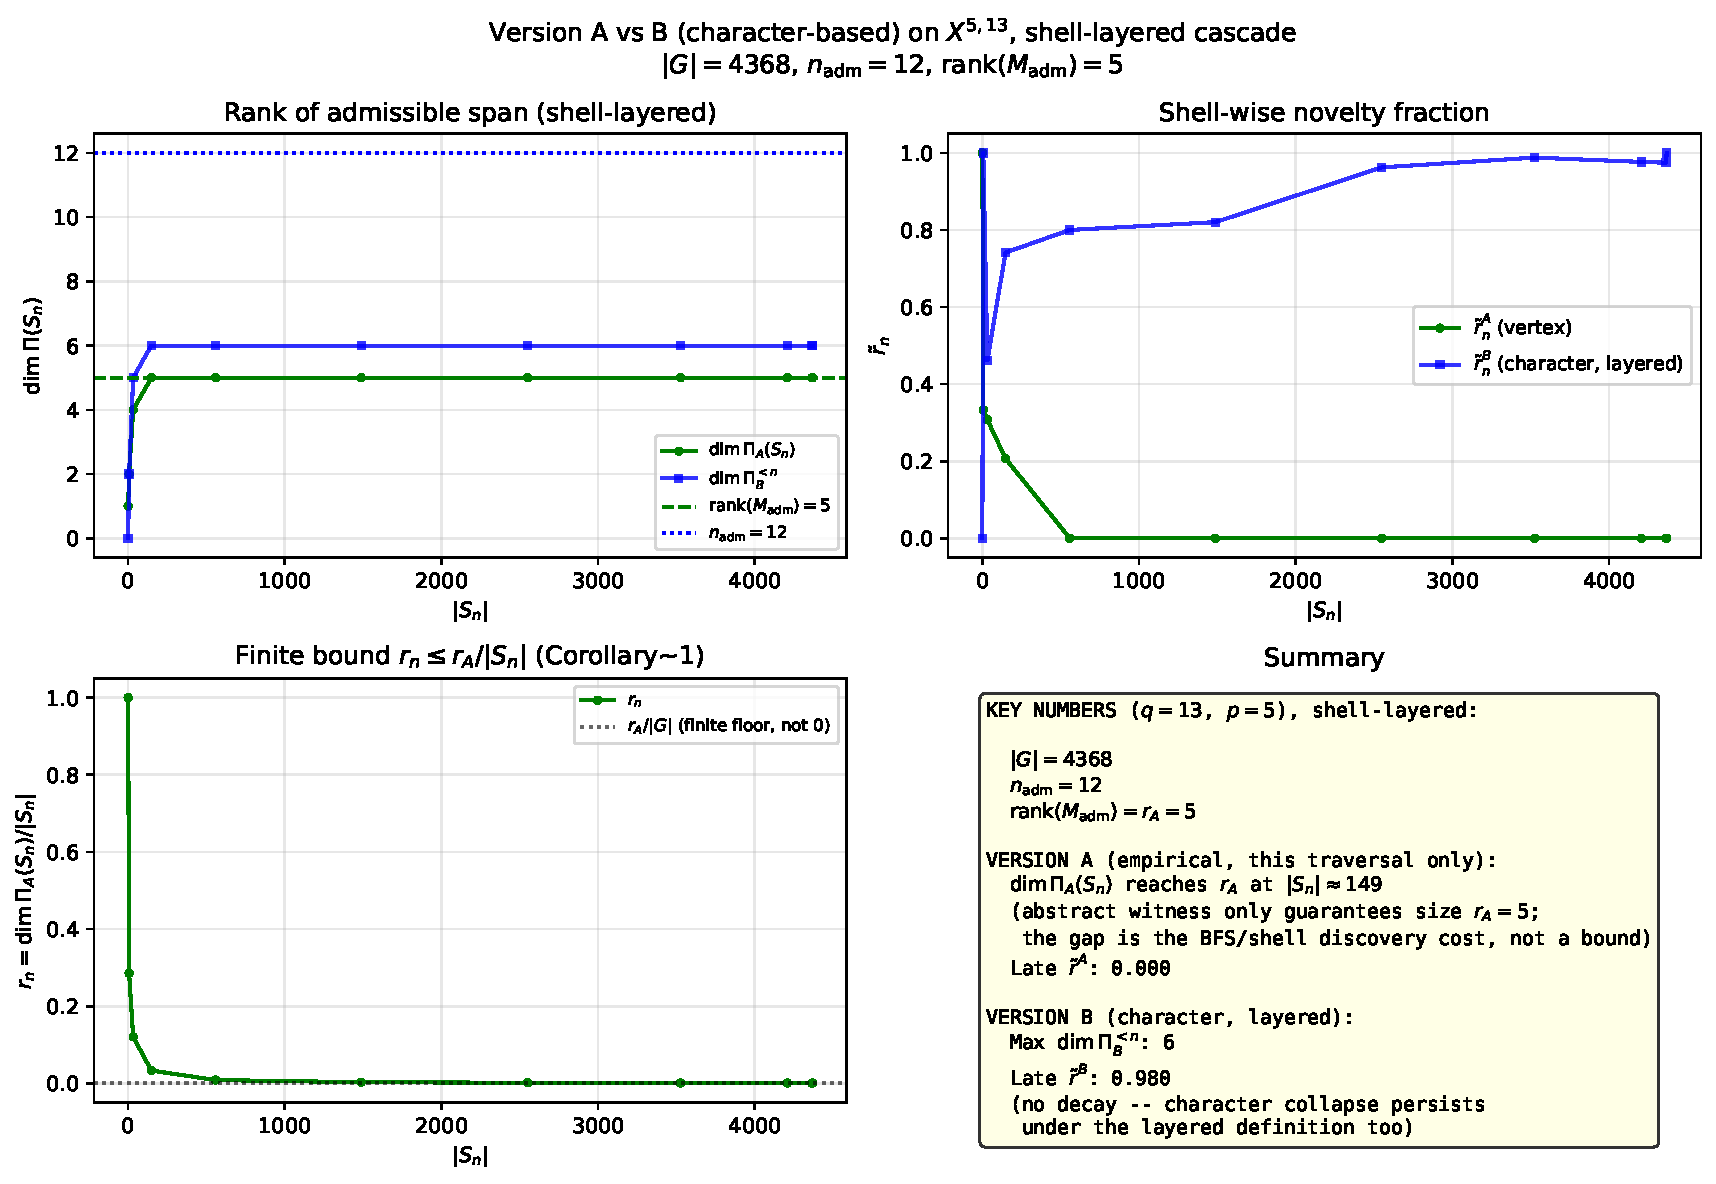
\includegraphics[width=\textwidth]{../code/fig1_A_vs_B}
        \caption{%
          Version~A vs.\ character-based Version~B on $X^{5,13}$ ($|G|=4368$, $n_{\adm}=12$,
          $\rank(M_{\adm})=r_A=5$), shell-layered cascade.
          \textit{Top left:} $\dim\Pi_A(S_n)$ reaches $r_A=5$ only at $|S_n|=149$, far above the
          abstract minimum (Remark~\ref{rem:numerical-A}); $\dim\Pi_B^{<n}$ plateaus at~6, well
          short of the ambient dimension~12.
          \textit{Top right:} the shell-wise novelty fraction $\tilde r_n^A$ falls to zero once the
          vertex span saturates; $\tilde r_n^B$ stays near~1 even after $\dim\Pi_B^{<n}$ has
          plateaued, because it measures whether a transition's fingerprint individually lies
          outside the prior span, not whether it adds new rank (Remark~\ref{rem:character-B-limitation}).
          \textit{Bottom:} the finite bound $r_n \le r_A/|S_n|$ of Corollary~\ref{cor:productivity-bound},
          which decays across the finite range $|S_n| \le |G|$ but does not tend to $0$ at fixed
          $q$.%
        }
        \label{fig:O5-A-vs-B}
      \end{figure}

      \begin{remark}[Vertex-based bound is a structural upper bound, not the final growth law]
        \label{rem:A-not-O5}
        The fingerprint $\piA(g)$ identifies group elements through conjugacy classes alone,
        capturing global projective redundancy but not transition-level novelty.
        Proposition~\ref{prop:vertex-admissible-saturation} is therefore a structural upper bound on
        the dimension of the admissible span, not yet a dynamical growth law for $\beta$, and not a
        statement about the size of any BFS-explored set at which that bound is achieved.
      \end{remark}

    \subsection{The transition-based admissible frontier}
      \label{subsec:transition-frontier}

      Proposition~\ref{prop:vertex-admissible-saturation} motivates a finer notion of admissible
      novelty sensitive to the \emph{transition} by which a boundary vertex is reached.
      Throughout this section, $S_n := \{g \in G : d(e,g) \le n\}$ denotes the ball of graph
      distance $n$ from a fixed origin vertex $e$, and $\mathrm{sh}_n := S_n \setminus S_{n-1}$
      (with $S_{-1} := \varnothing$) the corresponding shell.

      \begin{definition}[Transition-based admissible fingerprint, shell-layered]
        \label{def:transition-fingerprint}
        For $u \in G$, $s \in \mathcal{S}_p$, $v = u \cdot s$, define
        \[
          \piB(u \to v) := \bigl(\kap \, \chi_\rho(u) \, \chi_\rho(v)\bigr)_{\rho \in \Gadm}
          \in \R^{|\Gadm|}.
        \]
        For $n \ge 1$, let
        \[
          \PiBn{n} := \mathrm{span}_\R\bigl\{\piB(u\to v) :
            u \in \mathrm{sh}_{m-1},\, v = us \in \mathrm{sh}_m,\, s \in \mathcal{S}_p,\, 1 \le m < n\bigr\}
        \]
        be the span of transitions landing in shells \emph{strictly before} $n$, and define the
        layered transitional frontier of shell $n$ as
        \[
          \dB\, \mathrm{sh}_n := \bigl\{v \in \mathrm{sh}_n : \exists\, u \in \mathrm{sh}_{n-1},\,
            s \in \mathcal{S}_p,\; v = us,\; \piB(u\to v) \notin \PiBn{n}\bigr\}.
        \]
      \end{definition}

      \begin{remark}[Why the layering is not tautological]
        \label{rem:layering-nontautological}
        $\PiBn{n}$ is built exclusively from transitions landing in shells $0, \ldots, n-1$; no
        transition landing in $\mathrm{sh}_n$ contributes to it.
        Consequently $\dB\, \mathrm{sh}_n$ never tests a vector for membership in a span that was
        defined to contain it, unlike a definition that spans $\Pi_B(S_n)$ from \emph{all}
        transitions out of $S_n$ and then tests those same transitions against it, which is
        vacuous by construction.
        The definition depends only on graph distance from $e$, not on any BFS traversal order,
        parent choice, or insertion order within a shell.
      \end{remark}

      \begin{remark}[No general inclusion between the vertex and transition frontiers]
        \label{rem:frontier-hierarchy}
        $\piA(v)$ and $\piB(u\to v)$ are related only through the nonlinear (product) map
        $\chi_\rho(v) \mapsto \chi_\rho(u)\chi_\rho(v)$, not through a fixed linear transformation
        independent of $u$.
        No general inclusion $\dA S_n \subseteq \dB\, \mathrm{sh}_n$ (or the reverse) is established
        by this alone, and none is used below; each frontier is analysed on its own terms.
      \end{remark}

      \begin{remark}[Character degeneracy is necessary, not sufficient, for the observed non-decay]
        \label{rem:character-B-limitation}
        Definition~\ref{def:transition-fingerprint} uses only character data.
        On LPS graphs, the generators $\mathcal{S}_p$ lie in a single conjugacy class, so
        $\chi_\rho(s)$ is constant across $s \in \mathcal{S}_p$ for every $\rho$, and $\piB(u\to v)$
        therefore carries no information distinguishing which generator $s$ was used.
        This structural fact establishes only the absence of an explicit generator signal in the
        fingerprint; it does not by itself establish that the resulting span behaves like Version~A,
        or predict the specific plateau value at which $\dim\PiBn{n}$ saturates.
        That behaviour is a separate, numerically audited fact (Remark~\ref{rem:numerical-B}), not a
        consequence derived from the conjugacy-class argument alone.
        A relational refinement using representation matrices $\rho(s)$ is examined next.
      \end{remark}

      \begin{remark}[Numerical observation for the character-based fingerprint]
        \label{rem:numerical-B}
        Under the shell-layered definition, the character-based fingerprint was tested on
        $X^{5,13}$ ($\rank(\Madm)=5$, $|\Gadm|=12$) and $X^{5,29}$ ($\rank(\Madm)=9$, $|\Gadm|=28$).
        $\dim\PiBn{n}$ plateaus at $6$ for $X^{5,13}$ and at $14$ for $X^{5,29}$ --- in both cases
        short of the admissible ambient dimension $|\Gadm|$, though above $\rank(\Madm)$.
        The shell-wise novelty ratio $\tilde{r}_n^B$ nonetheless remains near $0.98$ (13) and $0.97$
        (29) after the initial shells: most individual transitions still fail the strict membership
        test even once the span itself has stopped growing.
        This dissociation is expected from Remark~\ref{rem:character-B-limitation}: $\tilde r_n^B$
        measures whether a single vector lies exactly in the current span, a much weaker condition
        than contributing a genuinely new dimension, so a high $\tilde r_n^B$ does not by itself
        indicate unbounded span growth --- as the plateau in $\dim\PiBn{n}$ shows directly.
        See Figure~\ref{fig:O5-versionB-saturation}.
      \end{remark}

      \begin{figure}[ht]
        \centering
        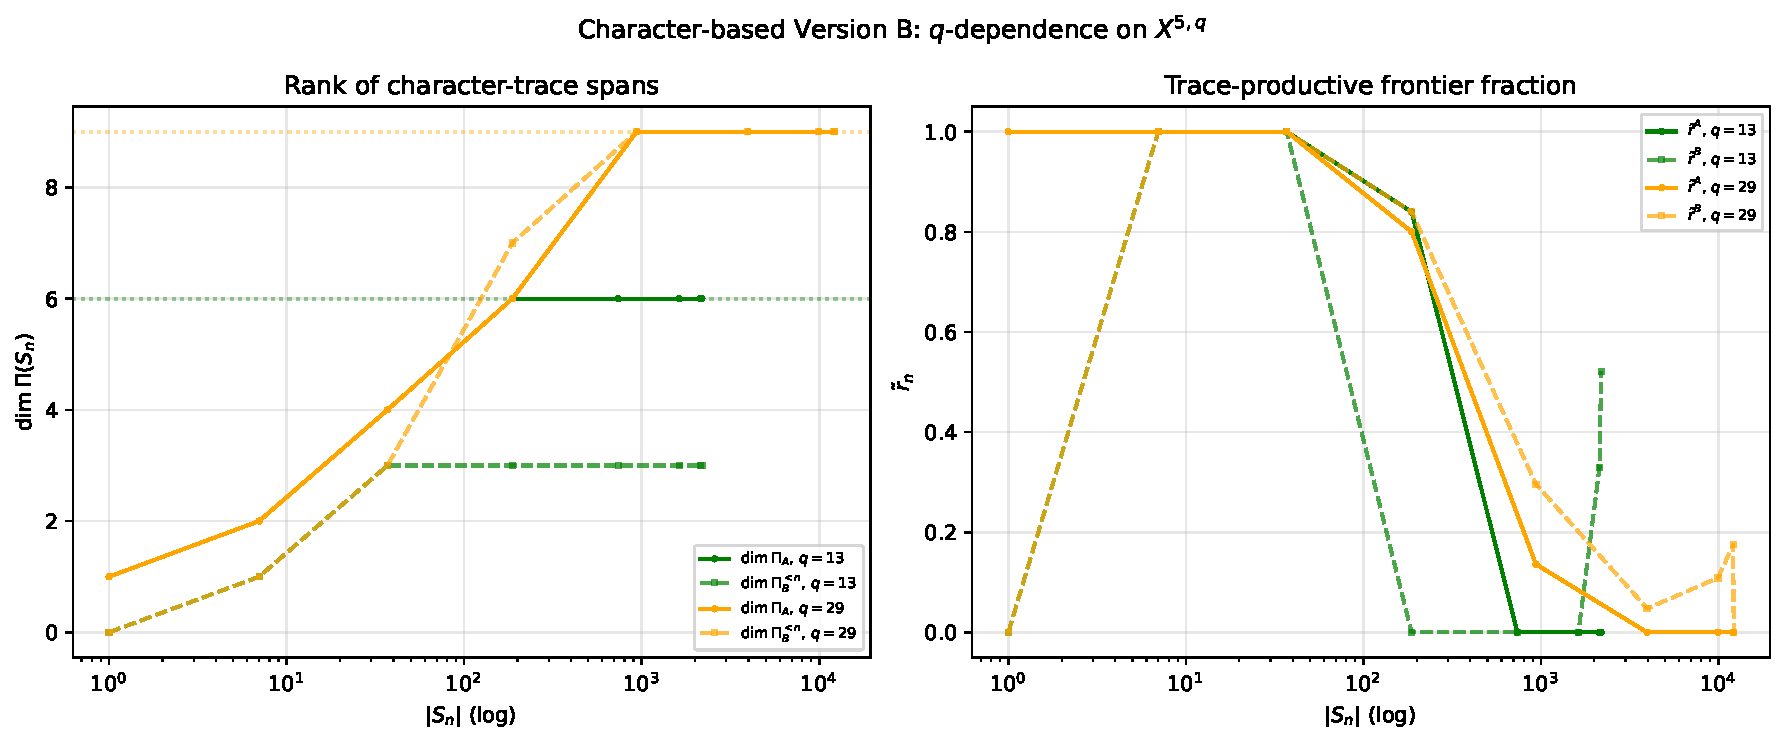
\includegraphics[width=\textwidth]{../code/fig2_versionB_sat}
        \caption{%
          $q$-dependence of the character-based, shell-layered fingerprint on $X^{5,q}$
          for $q \in \{13, 29\}$.
          \textit{Left:} $\dim\Pi_A$ saturates rapidly at $\rank(M_{\adm})$, while $\dim\Pi_B^{<n}$
          plateaus higher (6 of 12 for $q=13$; 14 of 28 for $q=29$) but still short of the ambient
          dimension.
          \textit{Right:} $\tilde r_n^B$ remains near $0.97$--$0.98$ for both values of $q$ even
          after the plateau, illustrating the dissociation of Remark~\ref{rem:numerical-B} between
          per-vector novelty and span growth.%
        }
        \label{fig:O5-versionB-saturation}
      \end{figure}

      \begin{remark}[Matrix-based transition fingerprint and the Steinberg prototype]
        \label{rem:matrix-B}
        A structurally adequate transition fingerprint should use representation operators:
        \[
          \Pi_\rho(u, s) \sim \rho(u)\,\rho(s), \qquad v = us.
        \]
        A prototype was implemented via the permutation action of $G$ on $\mathbb{P}^1(\F_q)$
        ($q+1$ points).
        Each element $g$ induces a permutation $\sigma_g$; the Steinberg projection
        $\tilde{\sigma}_g = \sigma_g - \mathrm{mean}(\sigma_g)$ lies in the $q$-dimensional Steinberg
        component.
        The fingerprint $\pi_B^{\mathrm{St}}(u\to v) = \tilde{\sigma}_u \odot \tilde{\sigma}_s
        \in \R^{q+1}$ is $O(q)$-dimensional and depends on $u$ and $s$ as matrices.
        Crucially, the LPS generators have six distinct Steinberg projections (while lying in
        only two conjugacy classes), breaking the character-level degeneracy.

        Under the shell-layered definition, numerical tests on $X^{5,q}$ for $q \in \{13, 17, 29\}$
        yield:
        \begin{itemize}[nosep]
\item Full ambient rank $q+1$ is reached at $|S^*_{\mathrm{St}}| = 33, 33, 151$ respectively, i.e.\
within graph-distance shells $2$--$3$ of the origin --- entirely inside the local, tree-like
regime where the LPS graph has not yet closed any short cycle around $e$, for every tested $q$.
\item The coincidence $|S^*_{\mathrm{St}}|=33$ for both $q=13$ and $q=17$ is explained by this
locality: shells $0$--$2$ have identical sizes $1, 6, 26$ for both graphs, since the local
$(p+1)$-regular tree structure around $e$ does not yet depend on $q$ at that radius.
\item Ratio $|S^*_{\mathrm{St}}|/|G| = 7.6\times10^{-3},\ 8.4\times10^{-4},\ 8.9\times10^{-4}$: it
shrinks with $q$, but the three-point sample is too coarse, and too dominated by the shared local
tree regime, to support a power-law fit $|S^*_{\mathrm{St}}| \sim q^\gamma$.
\item No pre-saturation regime survives from which an exponent could be extracted: saturation is
reached within the first two to three shells for every tested $q$, leaving fewer usable points than
any reasonable fit requires.
        \end{itemize}
        The Steinberg fingerprint therefore achieves genuine $q$-structural growth of its own
        saturation scale, but the resulting window is the opposite of what a quantitative extraction
        of $\betaeff$ would need: it closes almost immediately rather than opening one.
        See Figures~\ref{fig:O5-matB-variants} and~\ref{fig:O5-StElem-presat}.
      \end{remark}

      \begin{figure}[ht]
        \centering
        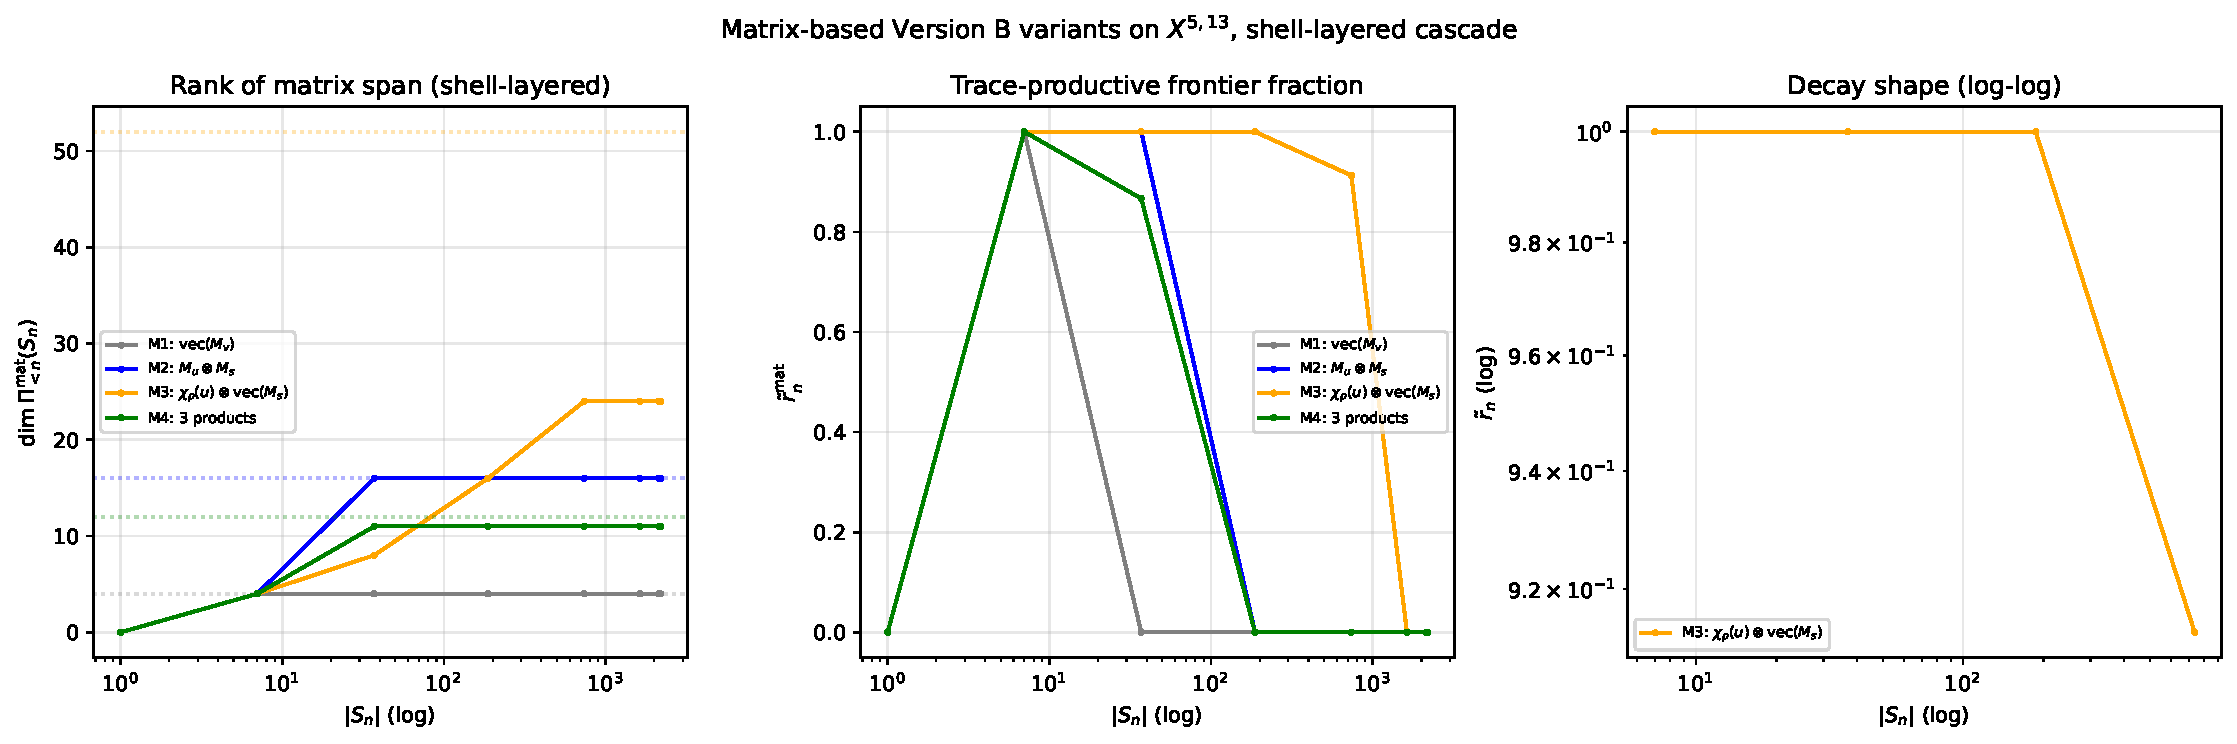
\includegraphics[width=\textwidth]{../code/fig3_matB_variants}
        \caption{%
          Matrix-based Version~B variants on $X^{5,13}$, shell-layered cascade.
          \textit{M1} ($\mathrm{vec}(M_v)$, $\dim=4$): trivial saturation at $|S_n|=7$, function of
          $v$ only.
          \textit{M2} ($M_u\otimes M_s$, $\dim=16$): full ambient saturation at $|S_n|=33$.
          \textit{M3} ($\chi_\rho(u)\otimes\mathrm{vec}(M_s)$, $\dim=48$): plateaus at $16$, short of
          the ambient dimension; character collapse persists as in the character-based fingerprint.
          \textit{M4} (three matrix products, $\dim=12$): plateaus at $11$ of $12$, essentially
          saturating like M2.
          Directional matrix structure is \emph{necessary} (M2/M4 vs.\ M3) but fixed ambient
          dimension is \emph{insufficient} (M2/M4 vs.\ Steinberg) for a $q$-structural mechanism.%
        }
        \label{fig:O5-matB-variants}
      \end{figure}

      \begin{figure}[ht]
        \centering
        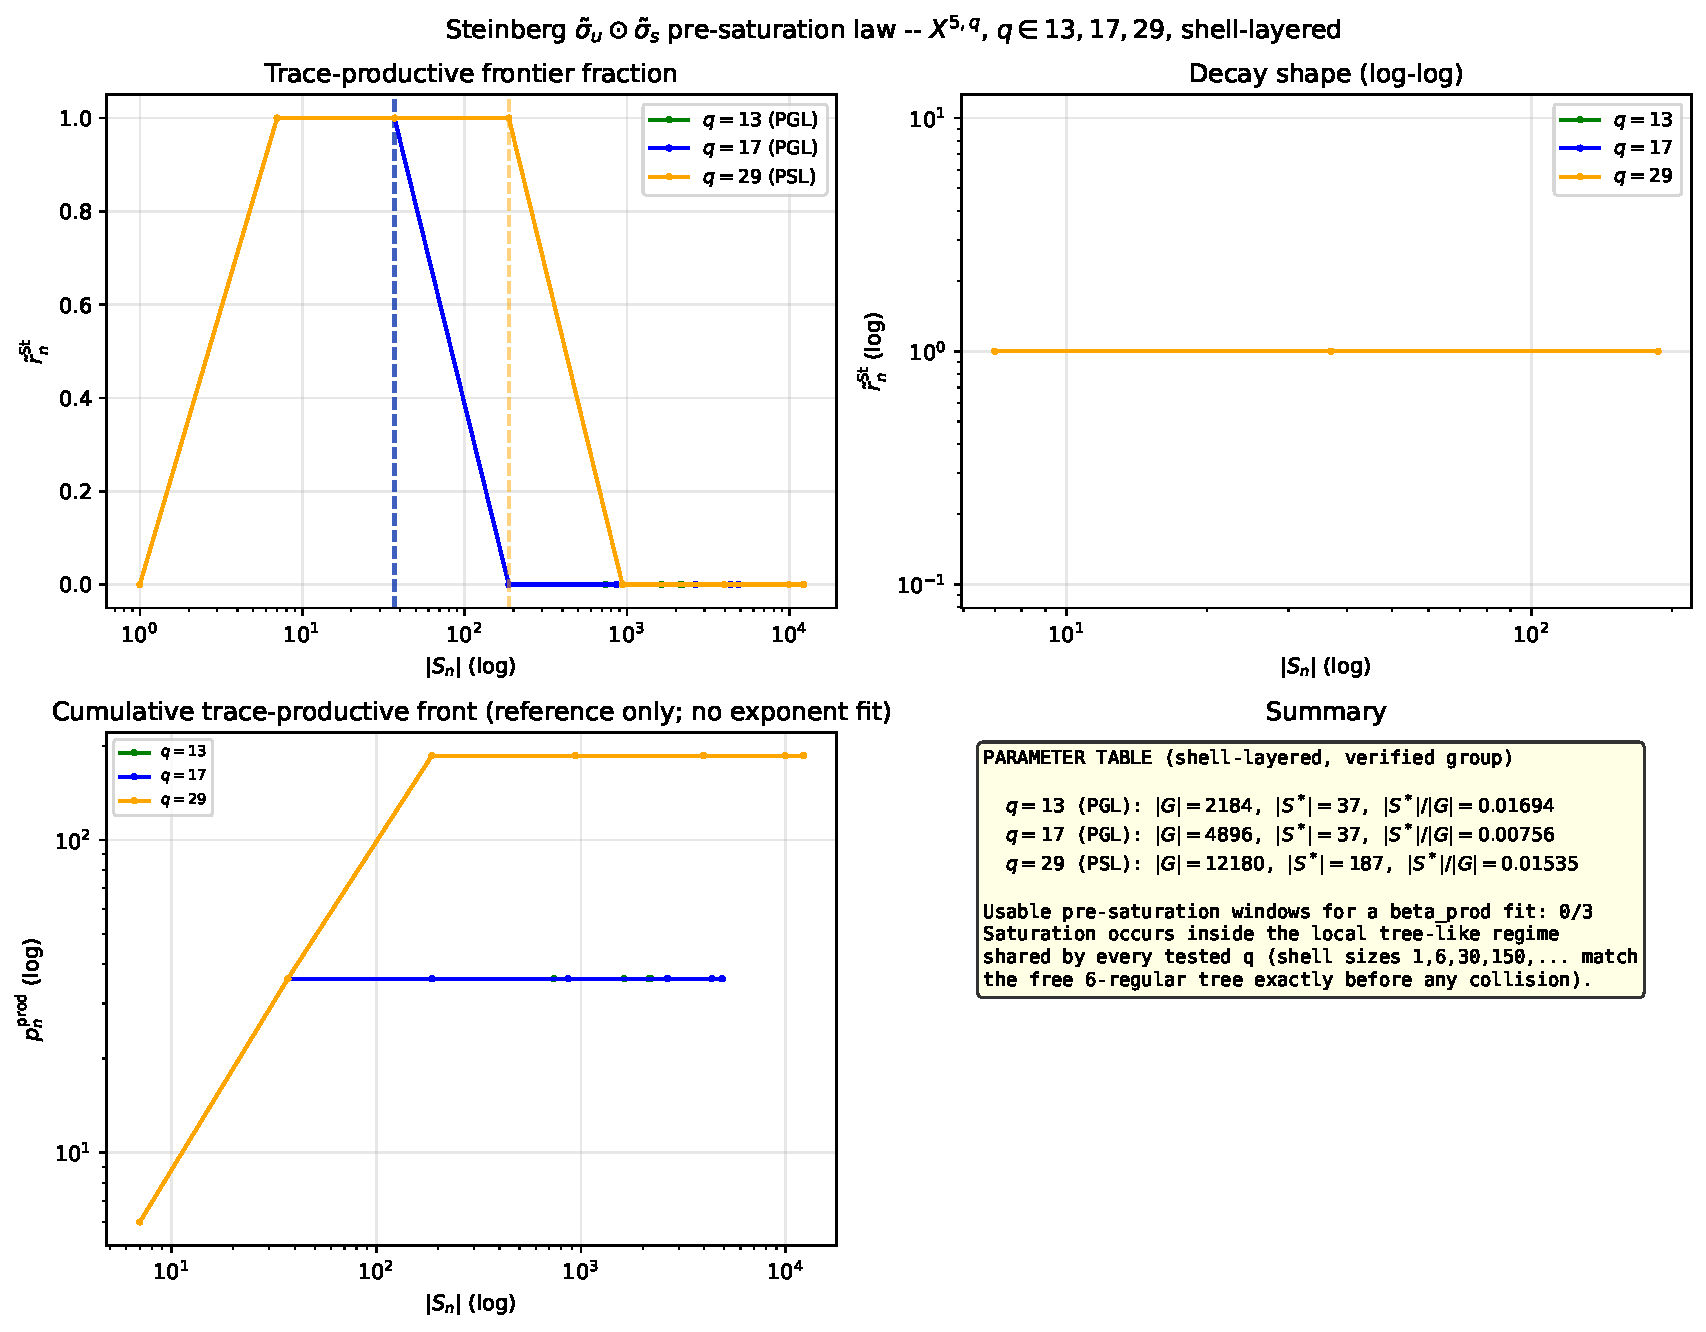
\includegraphics[width=\textwidth]{../code/fig4_StElem_presat}
        \caption{%
          Steinberg-based fingerprint $\pi_B^{\mathrm{St}}(u\to v) =
          \tilde\sigma_u \odot \tilde\sigma_s \in \R^{q+1}$ on $X^{5,q}$
          for $q\in\{13,17,29\}$, shell-layered cascade (Remark~\ref{rem:matrix-B}).
          \textit{Top left/right:} $\tilde r_n^{\mathrm{St}}$ falls to zero once the full ambient
          rank $q{+}1$ is reached, at $|S^*_{\mathrm{St}}| = 33, 33, 151$ (vertical dashed lines).
          \textit{Bottom left:} the cumulative admissible front $p_n^{\mathrm{prod}}$, shown for
          reference only: the pre-saturation range has too few shells for any exponent fit.
          \textit{Bottom right:} parameter table recording $|S^*_{\mathrm{St}}|$, $|S^*_{\mathrm{St}}|/|G|$,
          and the shared shell sizes $1,6,26$ responsible for the $q{=}13$/$q{=}17$ coincidence.%
        }
        \label{fig:O5-StElem-presat}
      \end{figure}

      \begin{remark}[Withdrawn conjecture: matrix-level admissible frontier decay]
        \label{rem:conjecture-withdrawn}
        The first version of this paper conjectured a matrix-based refinement of
        Definition~\ref{def:transition-fingerprint} for which
        \[
          \rtildeB := \frac{|\partial^{B,\mathrm{mat}}\,\mathrm{sh}_n|}{|\mathrm{sh}_n|}
          \xrightarrow{n \to \infty} 0,
          \qquad
          \frac{dp}{dn} \lesssim \rtildeB \cdot \sqrt{p(n)},
        \]
        and observed that a power-law ansatz $\rtildeB \sim p(n)^{-\alpha}$ integrates this to
        $\betaeff = 1/(1/2+\alpha)$, with the window $\betastar \in (0.09,0.13)$ requiring
        $\alpha \approx 9.5$.
        This conjecture is withdrawn as a candidate mechanism, for two independent reasons.
        First, none of the transition-based constructions examined here --- character-based,
        fixed-dimensional matrix, or Steinberg --- supplies a pre-saturation regime wide enough to
        even measure a decay exponent $\alpha$, let alone one near $9.5$
        (Remarks~\ref{rem:numerical-B} and~\ref{rem:matrix-B}); the conjecture's premise has no
        surviving candidate substrate in the present corpus.
        Second, the conjectured relation $\betaeff = 1/(1/2+\alpha)$ is exactly the functional form
        of the expander-derived capacity-to-rate conversion law that the companion Span-Growth
        Note~\cite{Beau2026sgn} proves has no native carrier when applied to a different
        admissibility substrate (the Heisenberg measurement graph), for the corpus-defined closure,
        frontier, pair observable, and exponent coordinates it audits.
        That result does not by itself refute the present $\PSL(2,\F_q)$ construction, which
        \cite{Beau2026sgn} does not address, but it removes any presumption that this functional form
        transfers natively between admissibility substrates, and so removes the conjecture's
        remaining motivation as a mechanism to pursue rather than merely a formal possibility.
      \end{remark}

    \subsection{Summary of contributions}
      \label{subsec:contributions-summary}

      \textbf{Claim 1 (Structural theorem).}
      The vertex-based admissible span has dimension $r_A \le \rank(\Madm) = O(q) \ll |G| = O(q^3)$,
      with a finite spanning witness of exactly that size
      (Proposition~\ref{prop:vertex-admissible-saturation}).
      This is proved from the representation theory of $\PSL(2,\F_q)$ alone; it makes no claim about
      how many vertices a graph exploration needs to reach such a witness, which the numerics show
      to be substantially larger (Corollary~\ref{cor:productivity-bound},
      Remark~\ref{rem:numerical-A}).

      \textbf{Claim 2 (Negative numerical result).}
      Under the non-tautological, shell-layered definition of Section~\ref{subsec:transition-frontier},
      the character-based transition fingerprint plateaus well short of the admissible ambient
      dimension on the tested LPS graphs (dimension $6$ of $12$ at $q=13$; $14$ of $28$ at $q=29$),
      although individual transitions keep testing as ``novel'' by the strict membership criterion.
      The single-conjugacy-class structure of the LPS generators explains the absence of an
      explicit generator signal in the fingerprint, but the specific plateau values are an
      independent numerical fact, not a consequence derived from that structural observation alone
      (Remarks~\ref{rem:character-B-limitation}--\ref{rem:numerical-B}).

      \textbf{Claim 3 (Negative proxy result).}
      Fixed-dimensional matrix fingerprints (M1, M2, M4) saturate their own small ambient dimension
      within a few dozen vertices, disqualifying them as $q$-structural mechanisms.
      The Steinberg prototype reaches its full $O(q)$-dimensional ambient rank within the first two
      to three graph-distance shells for every tested $q \in \{13,17,29\}$ --- inside the local,
      tree-like regime shared by all three graphs at that radius --- leaving no pre-saturation
      window from which any exponent could be extracted, for any of the tested $q$
      (Remark~\ref{rem:matrix-B}).

      \textbf{Consequence.}
      None of the three constructions supplies a viable mechanism for the smallness of $\betastar$:
      Claim~1 bounds a static dimension unrelated to exploration cost; Claim~2's character
      fingerprint plateaus without reaching the ambient dimension; Claim~3's proxies either
      saturate their own small ambient space or saturate the correct, growing ambient space too
      fast to measure anything.
      Whether a dynamical redundancy mechanism in a matrix-valued space of growing dimension could
      succeed where these constructions do not remains open; it is not established by the results
      above, and the specific conjectural form previously proposed for it is withdrawn
      (Remark~\ref{rem:conjecture-withdrawn}).

    \subsection{Structural implications}
      \label{subsec:structural-implications}

      Proposition~\ref{prop:vertex-admissible-saturation} is a group-theoretic fact following
      from the admissibility filter, with no appeal to dynamics.
      The dynamical question -- why is $\beta$ small? -- remains open after this paper's negative
      results (Section~\ref{subsec:contributions-summary}); Remark~\ref{rem:conjecture-withdrawn}
      records why the specific candidate rate law examined here does not currently constitute an
      answer.

      \begin{remark}[From dimensional saturation to dynamical redundancy]
        \label{rem:dim-to-dynred}
        Proposition~\ref{prop:vertex-admissible-saturation} confines vertex-level novelty to a
        space of dimension $\rank(\Madm) = O(q)$.
        By contrast, a matrix-level fingerprint $\rho(u)\rho(s)$ lives in $\End(V_\rho)$, so the
        full matrix-admissible space has dimension
        \[
          \sum_{\rho \in \Gadm} (\dim \rho)^2 = O(q^3) \sim |G|.
        \]
        No early dimensional saturation is structurally forced for the matrix-based Version~B.
        \emph{If} a suppression mechanism explaining $\betastar$ exists at the matrix level, it
        cannot arise from a dimensional constraint of the kind proved in
        Proposition~\ref{prop:vertex-admissible-saturation}, since the full matrix-admissible space
        is already $O(q^3) \sim |G|$: any such mechanism would have to be a genuinely dynamical
        redundancy phenomenon, not a representation-theoretic dimension bound.
        This paper does not establish that such a dynamical mechanism exists; it only rules out the
        dimensional route, and the constructions tested in
        Section~\ref{subsec:transition-frontier} do not supply a dynamical one either.
      \end{remark}

    \subsection{Outlook: toward O6}
      \label{subsec:outlook-O6}

      The hierarchy of mechanisms established in this paper is summarised in
      Table~\ref{tab:mechanisms}.

      \begin{table}[ht]
        \centering
        \caption{Hierarchy of admissible frontier mechanisms}
        \label{tab:mechanisms}
        \begin{tabular}{>{\itshape}l l p{7.5cm}}
          \toprule
          Version & Ambient dim & Status \\
          \midrule
          A (vertex, character) & $O(q)$ &
          Proposition~\ref{prop:vertex-admissible-saturation}: dimension bound $r_A=O(q)$ proved;
          empirical BFS witness at $|S_n|=149 \gg r_A=5$ ($q=13$) \\
          B (transition, character) & $O(q)$ &
          Plateaus short of ambient dimension ($6$ of $12$ at $q=13$; $14$ of $28$ at $q=29$)
          (Remark~\ref{rem:numerical-B}) \\
          B (transition, fixed matrix) & $O(1)$ &
          Saturates its own small ambient dimension within a few dozen vertices: not
          $q$-structural \\
          B (Steinberg, $\mathbb{P}^1$) & $O(q)$ &
          Saturates its full $q$-structural ambient dimension within shells $2$--$3$ for every
          tested $q$: no pre-saturation window survives \\
          \bottomrule
        \end{tabular}
      \end{table}

      \paragraph{Conclusion and outlook.}
        The admissible frontier analysis rules out several natural candidate mechanisms for the
        smallness of $\betastar$, without producing a positive one.
        At the vertex level, admissible novelty is provably confined to an $O(q)$-dimensional
        abstract span, but the empirical cost of a graph exploration reaching a witness of that
        span is substantially higher, and is not bounded by this paper's methods
        (Corollary~\ref{cor:productivity-bound}).
        At the transition level, the character-based fingerprint plateaus below the admissible
        ambient dimension without a clean interpretation as a structural mechanism, fixed-dimensional
        matrix proxies saturate their own small ambient space almost immediately, and the
        Steinberg-based fingerprint --- the one construction with genuinely $q$-structural ambient
        growth --- saturates so early, within the local tree-like regime shared by every tested $q$,
        that no pre-saturation window survives from which an exponent could be measured.

        These results collectively rule out the constructions examined here as mechanisms for the
        smallness of the cascade exponent; they do not establish what does explain it.
        The conjectural matrix-level redundancy law proposed in the first version of this paper is
        withdrawn (Remark~\ref{rem:conjecture-withdrawn}), both because no construction tested here
        supplies the regime in which it could be measured, and because its functional form
        coincides with a conversion law shown elsewhere in the corpus not to transfer natively
        between admissibility substrates.
        A viable mechanism, if one exists, remains to be found; this paper's contribution is to
        narrow the search by closing off the constructions above, not to identify the correct one.

  \section*{Acknowledgements}


  The author thanks the Cosmochrony programme for providing the theoretical scaffolding
  within which these computations are embedded.
  All numerical experiments were performed in Python using NumPy, SciPy, and Matplotlib.

  \section*{Data availability}

  All numerical computations reported here are reproducible from the Python scripts
  provided as supplementary material.
  The LPS graph construction follows the explicit generators of~\cite{Beau2026a1}
  (Section~9.6, $p=5$, $q \in \{13, 17, 29\}$).

  \clearpage
  \bibliographystyle{plain}
      \bibliography{cosmochrony-bibliography}

\end{document}
